\section{Teoría de Peano}

\subsection{El problema de Cauchy bajo continuidad y el fenómeno de no unicidad}

Hasta ahora hemos estudiado problemas de Cauchy bajo hipótesis Lipschitzianas, donde el Teorema de Picard-Lindelöf garantizaba no sólo la existencia local, sino la unicidad rigurosa y la prolongabilidad maximal de las soluciones. Sin embargo, en múltiples modelos físicos y biológicos la velocidad de variación no satisface una condición Lipschitziana uniforme.

Consideremos un problema de Cauchy general:
\[
    \begin{cases}
        u' = f(t, u) \\
        u(t_0) = u_0 \in \Omega \subset \mathbb{R}^N
    \end{cases}
\]
donde $J \subset \mathbb{R}$ es un intervalo abierto que contiene a $t_0$, $\Omega \subset \mathbb{R}^N$ es un abierto, y el campo $f: J \times \Omega \to \mathbb{R}^N$ se asume \textbf{únicamente continuo}:
\[
    f \in \mathcal{C}(J \times \Omega; \, \mathbb{R}^N)
\]
Bajo estas condiciones mínimas, el panorama analítico cambia drásticamente: \textbf{en general, no existe unicidad de soluciones}.

\ejemplo{
    \textbf{Pérdida de unicidad con campo no Lipschitziano:}

    Consideremos el problema autónomo escalar:
    \[
        \begin{cases}
            u' = \sqrt{|u|} \\
            u(0) = 0
        \end{cases}
    \]
    La función $f(u) = \sqrt{|u|}$ es continua en todo $\mathbb{R}$, pero su derivada:
    \[
        f'(u) = \frac{1}{2\sqrt{u}} \xrightarrow{u \to 0^+} +\infty
    \]
    no está acotada en ningún entorno del origen, por lo que $f$ no es Lipschitziana en $u = 0$.

    Este problema admite infinitas soluciones distintas. En primer lugar, la solución idénticamente nula:
    \[
        u_0(t) = 0 \qquad \forall t \in \mathbb{R}
    \]
    Además, para cualquier constante $c \geq 0$, la función:
    \[
        \varphi_c(t) = \begin{cases}
            0 & \text{si } t \leq c \\
            \dfrac{(t - c)^2}{4} & \text{si } t > c
        \end{cases}
    \]
    es de clase $\mathcal{C}^1(\mathbb{R})$ y satisface $\varphi_c(0) = 0$ y $\varphi_c'(t) = \sqrt{|\varphi_c(t)|}$ para todo $t \in \mathbb{R}$. Obtenemos así una familia no numerable de soluciones que se bifurcan a partir del punto de equilibrio.

    \begin{center}
    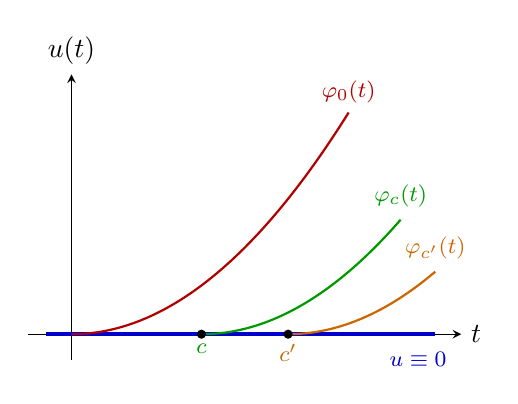
\begin{tikzpicture}[>=stealth, scale=1.1]
        % Ejes
        \draw[->] (-0.5,0) -- (4.5,0) node[right] {$t$};
        \draw[->] (0,-0.3) -- (0,3.0) node[above] {$u(t)$};
        
        % Solución idénticamente nula
        \draw[ultra thick, blue!80!black] (-0.3,0) -- (4.2,0);
        \node[below, blue!80!black, font=\footnotesize] at (4.0,-0.1) {$u \equiv 0$};
        
        % Solución para c = 0
        \draw[thick, red!70!black, domain=0:3.2, samples=60]
            plot (\x, {0.25*\x*\x});
        \node[above, red!70!black, font=\footnotesize] at (3.2,2.56) {$\varphi_0(t)$};
        
        % Solución para c = 1.5
        \draw[thick, green!60!black, domain=1.5:3.8, samples=60]
            plot (\x, {0.25*(\x - 1.5)*(\x - 1.5)});
        \node[above, green!60!black, font=\footnotesize] at (3.8,1.35) {$\varphi_c(t)$};
        \fill (1.5,0) circle (1.5pt);
        \node[below, green!60!black, font=\footnotesize] at (1.5,0) {$c$};
        
        % Solución para c = 2.5
        \draw[thick, orange!80!black, domain=2.5:4.2, samples=60]
            plot (\x, {0.25*(\x - 2.5)*(\x - 2.5)});
        \node[above, orange!80!black, font=\footnotesize] at (4.2,0.75) {$\varphi_{c'}(t)$};
        \fill (2.5,0) circle (1.5pt);
        \node[below, orange!80!black, font=\footnotesize] at (2.5,0) {$c'$};
    \end{tikzpicture}
    \end{center}
}

Para garantizar la existencia de al menos una solución bajo la sola hipótesis de continuidad, el principio de contracción de Banach resulta inoperante. La herramienta fundamental de Análisis Funcional que sustituye a las contracciones es el \textbf{Teorema de Ascoli-Arzelà} (desarrollado entre 1883 y 1895).

\subsection{Compacidad en espacios de Banach}

Sea $E$ un espacio de Banach (un espacio vectorial normado y completo sobre $\mathbb{R}$ con norma $\|\cdot\|_E$).

\begin{definición}[Conjunto relativamente compacto]
    Un subconjunto $X \subseteq E$ se dice \textbf{relativamente compacto} si su clausura $\overline{X}$ es un conjunto compacto en $(E, \|\cdot\|_E)$. En tal caso, $X$ es necesariamente acotado.
\end{definición}

La compacidad se caracteriza secuencialmente en espacios normados mediante el siguiente resultado clásico:

\begin{teorema}[Caracterización de relativa compacidad]
    Sea $E$ un espacio de Banach y $X \subseteq E$. Las siguientes afirmaciones son equivalentes:
    \begin{itemize}
        \item $X$ es relativamente compacto en $E$.
        \item De toda sucesión infinita $\{x_n\}_{n \geq 1} \subset X$ se puede extraer una subsucesión $\{x_{n_m}\}_{m \geq 1}$ convergente en $E$ a un punto del cierre $\overline{X}$.
    \end{itemize}
\end{teorema}

\textbf{El caso de dimensión finita ($E = \mathbb{R}^N$):}

En espacios euclídeos de dimensión finita, el Teorema de Bolzano-Weierstrass establece que todo conjunto acotado posee subsucesiones convergentes:
\[
    X \subset \mathbb{R}^N \text{ relativamente compacto} \iff \overline{X} \text{ es cerrado y acotado} \iff X \text{ es acotado}
\]
Por consiguiente, en $\mathbb{R}^N$ los conjuntos relativamente compactos son exactamente los conjuntos acotados.

\medskip

\textbf{El problema en dimensión infinita:}

Consideremos un subconjunto compacto no vacío $K \subset \mathbb{R}^M$ y el espacio vectorial de las funciones continuas $\mathcal{C}(K; \, \mathbb{R}^N)$ dotado de la norma del supremo:
\[
    \|u\|_\infty = \max_{x \in K} \|u(x)\|
\]
El espacio $(\mathcal{C}(K; \, \mathbb{R}^N), \, \|\cdot\|_\infty)$ es un espacio de Banach de dimensión infinita. Surge de manera natural la cuestión: \textit{¿cuáles son los subconjuntos $\mathcal{F} \subset \mathcal{C}(K; \, \mathbb{R}^N)$ relativamente compactos? ¿Basta que una familia sea acotada?}

La respuesta es rotundamente \textbf{NO}: en dimensión infinita existen familias acotadas que no admiten ninguna subsucesión convergente.

\subsubsection{Contraejemplo: insuficiencia de la acotación uniforme}

Para ilustrar este fenómeno, consideremos en el espacio $\mathcal{C}([0, 1]; \, \mathbb{R})$ la sucesión de funciones potenciales:
\[
    f_n: [0, 1] \to \mathbb{R}, \qquad f_n(t) = t^n \quad (n \geq 1)
\]
Cada función $f_n$ es continua en $[0, 1]$, y la familia $\mathcal{F} = \{f_n\}_{n \geq 1}$ está acotada en norma del supremo:
\[
    |f_n(t)| = |t^n| \leq 1 \implies \|f_n\|_{\infty, [0, 1]} = 1 \qquad \forall n \geq 1
\]
Analicemos el límite puntual de $f_n$ cuando $n \to \infty$:
\[
    f(t) = \lim_{n \to \infty} t^n = \begin{cases}
        0 & \text{si } t \in [0, 1) \\
        1 & \text{si } t = 1
    \end{cases}
\]
La función límite $f(t)$ presenta una discontinuidad inevitable de salto en $t = 1$.

\begin{proposición}[No compacidad de la familia de potencias]
    La familia $\mathcal{F} = \{f_n\}_{n \geq 1} = \{t^n\}_{n \geq 1}$ no es relativamente compacta en $\mathcal{C}([0, 1]; \, \mathbb{R})$.
\end{proposición}

\begin{proof}
    Razonemos por reducción al absurdo. Supongamos que $\mathcal{F}$ fuera relativamente compacta en $\mathcal{C}([0, 1]; \, \mathbb{R})$. Entonces existiría una subsucesión $\{f_{n_m}\}_{m \geq 1} \subset \mathcal{F}$ convergente en la norma $\|\cdot\|_\infty$ a alguna función $g \in \mathcal{C}([0, 1]; \, \mathbb{R})$:
    \[
        \lim_{m \to \infty} \|f_{n_m} - g\|_\infty = 0
    \]
    La convergencia uniforme implica que $f_{n_m}(t)$ converge puntualmente a $g(t)$ para todo $t \in [0, 1]$:
    \[
        g(t) = \lim_{m \to \infty} f_{n_m}(t) \qquad \forall t \in [0, 1]
    \]
    Por otra parte, como cualquier subsucesión de una sucesión convergente comparte el mismo límite puntual, se tiene forzosamente que $g(t) = f(t)$ para todo $t \in [0, 1]$, siendo $f$ la función discontinua obtenida anteriormente:
    \[
        g(t) = \begin{cases}
            0 & \text{si } t \in [0, 1) \\
            1 & \text{si } t = 1
        \end{cases}
    \]
    Esto entra en contradicción directa con el hecho de que $g \in \mathcal{C}([0, 1]; \, \mathbb{R})$. Concluimos que de la sucesión acotada $\{f_n\}$ no puede extraerse ninguna subsucesión convergente en $\mathcal{C}([0, 1]; \, \mathbb{R})$, luego $\mathcal{F}$ no es relativamente compacta.
\end{proof}

\begin{center}
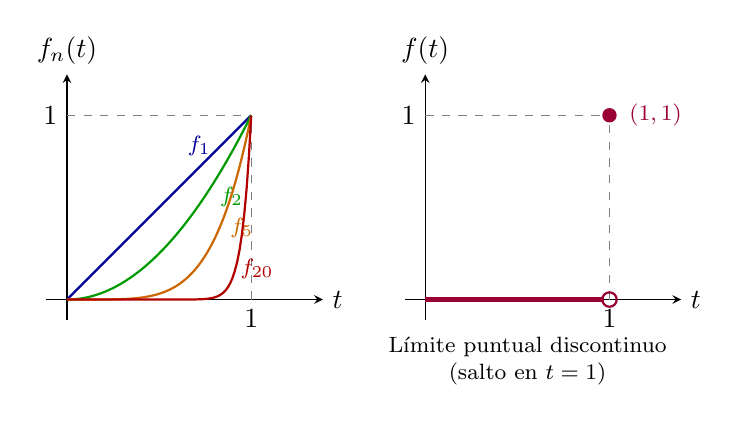
\begin{tikzpicture}[>=stealth, scale=1.3]
    % Ejes
    \draw[->] (-0.2,0) -- (2.5,0) node[right] {$t$};
    \draw[->] (0,-0.2) -- (0,2.2) node[above] {$f_n(t)$};
    
    % Cuadrado unitario
    \draw[dashed, gray] (1.8,0) node[below, black] {$1$} -- (1.8,1.8);
    \draw[dashed, gray] (0,1.8) node[left, black] {$1$} -- (1.8,1.8);
    
    % Curvas t^n
    \draw[thick, blue!60!black, domain=0:1.8, samples=50]
        plot (\x, {\x});
    \node[left, blue!60!black, font=\footnotesize] at (1.5,1.5) {$f_1$};
    
    \draw[thick, green!60!black, domain=0:1.8, samples=50]
        plot (\x, {(\x/1.8)^2 * 1.8});
    \node[right, green!60!black, font=\footnotesize] at (1.4,1.0) {$f_2$};
    
    \draw[thick, orange!80!black, domain=0:1.8, samples=60]
        plot (\x, {(\x/1.8)^5 * 1.8});
    \node[right, orange!80!black, font=\footnotesize] at (1.5,0.7) {$f_5$};
    
    \draw[thick, red!70!black, domain=0:1.8, samples=80]
        plot (\x, {(\x/1.8)^20 * 1.8});
    \node[right, red!70!black, font=\footnotesize] at (1.6,0.3) {$f_{20}$};
    
    % Límite puntual discontinuo
    \begin{scope}[xshift=3.5cm]
        \draw[->] (-0.2,0) -- (2.5,0) node[right] {$t$};
        \draw[->] (0,-0.2) -- (0,2.2) node[above] {$f(t)$};
        \draw[dashed, gray] (1.8,0) node[below, black] {$1$} -- (1.8,1.8);
        \draw[dashed, gray] (0,1.8) node[left, black] {$1$} -- (1.8,1.8);
        
        \draw[ultra thick, purple!80!black] (0,0) -- (1.75,0);
        \draw[purple!80!black, thick] (1.8,0) circle (2pt);
        \fill[purple!80!black] (1.8,1.8) circle (2pt);
        \node[right, purple!80!black, font=\footnotesize] at (1.9,1.8) {$(1, 1)$};
        \node[font=\footnotesize, align=center] at (1.0,-0.6) {Límite puntual discontinuo\\(salto en $t = 1$)};
    \end{scope}
\end{tikzpicture}
\end{center}

\subsection{Equicontinuidad y el Teorema de Ascoli-Arzelà}

Para evitar que las funciones de una familia oscilen o se empinen indefinidamente (como ocurría con $t^n$ cerca de $t = 1$), es imprescindible imponer que la continuidad sea simultánea y homogénea para todos los miembros de la familia.

\begin{definición}[Familia equicontinua]
    Sea $K \subset \mathbb{R}^M$ compacto. Un subconjunto $\mathcal{F} \subset \mathcal{C}(K; \, \mathbb{R}^N)$ se dice \textbf{equicontinuo} si:
    \[
        \forall \varepsilon > 0, \; \exists \delta > 0 \quad \text{tal que} \quad \forall x, y \in K, \; \|x - y\| < \delta \implies \|f(x) - f(y)\| < \varepsilon \quad \forall f \in \mathcal{F}
    \]
\end{definición}

Es esencial subrayar que el módulo de continuidad $\delta$ depende exclusivamente de $\varepsilon$, siendo independiente tanto de los puntos concretos $x, y \in K$ como de la función elegida $f \in \mathcal{F}$.

\begin{lema}[Equicontinuidad mediante condición de Lipschitz uniforme]
    Sea $K \subset \mathbb{R}^M$ compacto y $\mathcal{F} \subset \mathcal{C}(K; \, \mathbb{R}^N)$ una familia de funciones globalmente Lipschitzianas en $K$ con una constante de Lipschitz común $L > 0$:
    \[
        \|f(x) - f(y)\| \leq L \|x - y\| \qquad \forall x, y \in K, \quad \forall f \in \mathcal{F}
    \]
    Entonces $\mathcal{F}$ es equicontinua.
\end{lema}

\begin{proof}
    Dado cualquier $\varepsilon > 0$, tomamos $\delta = \frac{\varepsilon}{L} > 0$. Para cualesquiera $x, y \in K$ con $\|x - y\| < \delta$ y cualquier $f \in \mathcal{F}$:
    \[
        \|f(x) - f(y)\| \leq L \|x - y\| < L \delta = L \frac{\varepsilon}{L} = \varepsilon
    \]
    lo que prueba que $\mathcal{F}$ es equicontinua.
\end{proof}

\begin{observación}[Aplicación a sucesiones de soluciones de ecuaciones diferenciales]
    Consideremos un intervalo compacto $J = [t_0, t_0 + T]$ y una sucesión de trayectorias $\{u_n\}_{n \geq 1} \subset \mathcal{C}(J; \, \mathbb{R}^N)$ que satisfacen:
    \[
        u_n'(t) = f(t, u_n(t)) \qquad \forall t \in J, \quad \forall n \geq 1
    \]
    donde $f: J \times \mathbb{R}^N \to \mathbb{R}^N$ es continua. Si la familia $\{u_n\}$ está acotada en norma del supremo:
    \[
        \sup_{n \geq 1} \|u_n\|_\infty \leq R
    \]
    entonces todos los pares $(t, u_n(t))$ pertenecen al conjunto compacto $K_0 = J \times \overline{B_R(0)}$. Por el Teorema de Weierstrass, $f$ está acotada en $K_0$:
    \[
        C = \max_{(t, x) \in K_0} \|f(t, x)\| < +\infty
    \]
    En consecuencia, la velocidad está uniformemente acotada:
    \[
        \|u_n'(t)\| = \|f(t, u_n(t))\| \leq C \qquad \forall t \in J, \quad \forall n \geq 1
    \]
    Integrando entre cualesquiera $s, t \in J$:
    \[
        \|u_n(t) - u_n(s)\| = \left\| \int_s^t u_n'(\tau)\, d\tau \right\| \leq \left| \int_s^t \|u_n'(\tau)\|\, d\tau \right| \leq C |t - s|
    \]
    Por el lema anterior, $\{u_n\}_{n \geq 1}$ es automáticamente una familia equicontinua en $\mathcal{C}(J; \, \mathbb{R}^N)$.
\end{observación}

\subsubsection{El Teorema de Ascoli-Arzelà}

El Teorema de Ascoli-Arzelà culmina esta teoría proporcionando la caracterización completa y definitiva de los conjuntos compactos en espacios de funciones continuas.

\begin{teorema}[Teorema de Ascoli-Arzelà]
    Sea $K \subset \mathbb{R}^M$ un subconjunto compacto y $\mathcal{F} \subset \mathcal{C}(K; \, \mathbb{R}^N)$. Las siguientes afirmaciones son equivalentes:
    \begin{itemize}
        \item $\mathcal{F}$ es relativamente compacto en $(\mathcal{C}(K; \, \mathbb{R}^N), \, \|\cdot\|_\infty)$.
        \item $\mathcal{F}$ es uniformemente acotado y equicontinuo en $\mathcal{C}(K; \, \mathbb{R}^N)$.
    \end{itemize}
\end{teorema}

\begin{proof}
    Demostramos la implicación directa: que la relativa compacidad implica necesariamente la acotación uniforme y la equicontinuidad de la familia $\mathcal{F}$.

    Supongamos que $\mathcal{F}$ es relativamente compacto en $\mathcal{C}(K; \, \mathbb{R}^N)$. Por definición, su clausura $\overline{\mathcal{F}}$ es un subconjunto compacto del espacio de Banach $(\mathcal{C}(K; \, \mathbb{R}^N), \|\cdot\|_\infty)$.

    \medskip

    \textbf{1. Acotación uniforme:}

    Para el radio fijo $\varepsilon = 1$, consideramos el recubrimiento abierto de $\overline{\mathcal{F}}$ por bolas abiertas:
    \[
        \overline{\mathcal{F}} \subset \bigcup_{f \in \overline{\mathcal{F}}} B_1(f)
    \]
    Por la compacidad de $\overline{\mathcal{F}}$, existe una subfamilia finita de centros $\{f_1, f_2, \dots, f_q\} \subset \overline{\mathcal{F}}$ tal que:
    \[
        \overline{\mathcal{F}} \subset \bigcup_{j=1}^q B_1(f_j)
    \]
    Sea ahora $f \in \overline{\mathcal{F}}$ arbitraria. Existe algún índice $j \in \{1, \dots, q\}$ para el cual $f \in B_1(f_j)$, es decir, $\|f - f_j\|_\infty < 1$. Aplicando la desigualdad triangular:
    \[
        \|f\|_\infty \leq \|f - f_j\|_\infty + \|f_j\|_\infty < 1 + \|f_j\|_\infty \leq 1 + \max_{1 \leq k \leq q} \|f_k\|_\infty \equiv R
    \]
    Como $R$ es una constante finita que no depende de la función $f$, se tiene:
    \[
        \overline{\mathcal{F}} \subset B_R(0)
    \]
    Por tanto, $\overline{\mathcal{F}}$ y en consecuencia $\mathcal{F}$ están uniformemente acotados en $\mathcal{C}(K; \, \mathbb{R}^N)$.

    \medskip

    \textbf{2. Equicontinuidad:}

    Razonamos por reducción al absurdo. Supongamos que la familia $\mathcal{F}$ \textbf{no} es equicontinua en $K$. 

    Negando la definición de equicontinuidad, existe un $\varepsilon_0 > 0$ tal que para todo $\delta > 0$, es posible encontrar dos puntos $x, y \in K$ y una función $f \in \mathcal{F}$ que verifican $\|x - y\| < \delta$ pero $\|f(x) - f(y)\| \geq \varepsilon_0$.

    Tomando sucesivamente $\delta_n = \frac{1}{n}$ para cada $n \in \mathbb{N}$, existen puntos $x_n, y_n \in K$ y funciones $f_n \in \mathcal{F}$ tales que:
    \[
        \|x_n - y_n\| < \frac{1}{n} \qquad \text{y} \qquad \|f_n(x_n) - f_n(y_n)\| \geq \varepsilon_0 \qquad \forall n \geq 1
    \]
    Consideremos la sucesión de ternas $\{(x_n, y_n, f_n)\}_{n \geq 1}$ en el espacio producto:
    \[
        (x_n, y_n, f_n) \in K \times K \times \overline{\mathcal{F}}
    \]
    Como $K$ es compacto en $\mathbb{R}^M$ y $\overline{\mathcal{F}}$ es compacto en $(\mathcal{C}(K; \, \mathbb{R}^N), \|\cdot\|_\infty)$, el producto cartesiano:
    \[
        K \times K \times \overline{\mathcal{F}}
    \]
    es un espacio métrico compacto (por el Teorema de Tychonoff en espacios métricos). Por compacidad secuencial, podemos extraer una subsucesión convergente:
    \[
        (x_{n_m}, y_{n_m}, f_{n_m}) \xrightarrow{m \to \infty} (x, y, f) \in K \times K \times \overline{\mathcal{F}}
    \]
    En consecuencia, convergen sus componentes individuales:
    \[
        x_{n_m} \xrightarrow{m \to \infty} x, \qquad y_{n_m} \xrightarrow{m \to \infty} y, \qquad \lim_{m \to \infty} \|f_{n_m} - f\|_\infty = 0
    \]
    Además, pasando al límite en la distancia entre $x_{n_m}$ e $y_{n_m}$:
    \[
        \|x - y\| = \lim_{m \to \infty} \|x_{n_m} - y_{n_m}\| \leq \lim_{m \to \infty} \frac{1}{n_m} = 0 \implies x = y
    \]
    Descomponemos ahora la diferencia $\|f_{n_m}(x_{n_m}) - f_{n_m}(y_{n_m})\|$ sumando y restando los valores de la función límite $f$ e intercalando por la desigualdad triangular:
    \[
        \|f_{n_m}(x_{n_m}) - f_{n_m}(y_{n_m})\| \leq \|f_{n_m}(x_{n_m}) - f(x_{n_m})\| + \|f(x_{n_m}) - f(y_{n_m})\| + \|f(y_{n_m}) - f_{n_m}(y_{n_m})\|
    \]
    Acotando los términos extremos mediante la norma del supremo:
    \[
        \varepsilon_0 \leq \|f_{n_m}(x_{n_m}) - f_{n_m}(y_{n_m})\| \leq 2 \|f_{n_m} - f\|_\infty + \|f(x_{n_m}) - f(y_{n_m})\|
    \]
    Analizamos el comportamiento de cada término cuando $m \to \infty$:
    \begin{itemize}
        \item Por la convergencia uniforme de la subsucesión $\{f_{n_m}\}$ en $\mathcal{C}(K; \, \mathbb{R}^N)$:
        \[
            \lim_{m \to \infty} \|f_{n_m} - f\|_\infty = 0
        \]
        \item Como $f \in \mathcal{C}(K; \, \mathbb{R}^N)$ es una función continua en el compacto $K$ y tanto $x_{n_m}$ como $y_{n_m}$ convergen al mismo punto común $x = y$:
        \[
            \lim_{m \to \infty} \|f(x_{n_m}) - f(y_{n_m})\| = \|f(x) - f(x)\| = 0
        \]
    \end{itemize}
    Tomando el límite cuando $m \to \infty$ en la desigualdad anterior, obtenemos:
    \[
        \varepsilon_0 \leq 0 + 0 = 0
    \]
    lo que contradice flagrantemente que $\varepsilon_0 > 0$.

    Esta contradicción demuestra que la hipótesis de no equicontinuidad es insostenible. Por consiguiente, $\mathcal{F}$ es forzosamente equicontinua en $K$.
\end{proof}

% LO ANTERIOR A ESTO ESTÁ GENERADO HASTA EL MIÉRCOLES, EN EL ARCHIVO AUXILIAR, REVISAR SI ESTÁ BIEN COHESIONADO CON LO QUE VIENE A CONTINUACIÓN

Para demostrarlo seguiremos 3 etapas:

\begin{enumerate}
    \item Con la compacidad de $\mathcal{K}$ veremos que $\exists D = \{d_n\}_{n \in \mathbb{N}} \subset \mathcal{K}$ tal que $\overline{D} = \mathcal{K}$, es decir, $D$ es denso en $\mathcal{K}$.
    \item Con la acotación de $\mathcal{F}$ veremos que existe una subsucesión de funciones $\{g_n\}_{n \in \mathbb{N}}$ de $\{f_n\}_{n \in \mathbb{N}}$ convergente en $D$.
    \item Con la equicontinuidad de $\mathcal{F}$ veremos que la subsucesión $\{g_n\}_{n \in \mathbb{N}}$ es de Cauchy en $C(\mathcal{K}, \mathbb{R}^n)$ y por tanto convergente en $C(\mathcal{K}, \mathbb{R}^n)$.
\end{enumerate}

\begin{proof}
    Vayamos etapa por etapa:
    \begin{enumerate}
        \item \textbf{Etapa 1:} Sabemos que, por la compacidad de $\mathcal{K}$:
        \[
            \mathcal{K} \subset \bigcup_{x \in \mathcal{K}} B_{\frac{1}{n}}(x) \quad \forall n \in \mathbb{N} \implies
            \exists \{x_1, \dots, x_{k_n}\} \subset \mathcal{K} : \mathcal{K} \subset \bigcup_{i=1}^{k_n} B_{\frac{1}{n}}(x_i) \quad \forall n \in \mathbb{N}
        \]
        Y por tanto, tomemos $D = \{x_i\}_{i=1}^{i=m} \subset \mathcal{K}$, que es denso en $\mathcal{K}$.\\

        Además, tomando cualquier $x \in \mathcal{K}$, $\exists \{x_{i_n}\}_{n \in \mathbb{N}} \subset D$ tal que:
        \[
            x \in B_{\frac{1}{n}}(x_{i_n}) \implies
            d(x, x_{i_n}) < \frac{1}{n} \implies
            \lim_{n \to \infty} d(x, x_{i_n}) = 0 \implies
            \lim_{n \to \infty} x_{i_n} = x
        \]
        \item \textbf{Etapa 2:} Sea $\{f_n\}_{n \in \mathbb{N}} \subset \mathcal{F}$ una sucesión de funciones, y sea $D = \{d_n\}_{n \in \mathbb{N}}$ el conjunto denso en $\mathcal{K}$ que hemos construido en la etapa 1.\\
        
        Como $\mathcal{F}$ es acotado, $\exists M > 0$ tal que:
        \[
            \|f_n\|_\infty \leq M \quad \forall n \in \mathbb{N} \implies
            \max_{x \in \mathcal{K}} |f_n(x)| \leq M \implies
            \| f_n(x) \| \leq M \quad \forall n \in \mathbb{N}, \forall x \in \mathcal{K}
        \]

        Por lo tanto, $\{f_n(d_1)\}_{n \in \mathbb{N}}$ es una sucesión acotada en $\mathbb{R}^n$, y por el teorema de Bolzano-Weierstrass, $\exists \{f_n^1\}_{n \in \mathbb{N}}$ una subsucesión convergente de $\{f_n(d_1)\}_{n \in \mathbb{N}}$, tal que:
        \[
            \lim_{n \to \infty} f_n^1(d_1) = L_1
        \]

        Así, podemos tener una sucesión de funciones $f_1^1, f_2^1, \dots$ convergente en $d_1$.\\

        Ahora, como $\{f_n^1(d_2)\}_{n \in \mathbb{N}}$ es una sucesión acotada en $\mathbb{R}^n$, $\exists \{f_n^2\}_{n \in \mathbb{N}}$ una subsucesión convergente de $\{f_n^1(d_2)\}_{n \in \mathbb{N}}$, tal que:
        \[
            \lim_{n \to \infty} f_n^2(d_2) = L_2
        \]

        Y así, tendríamos que la sucesión de funciones $f_1^2, f_2^2, \dots$ converge en $d_1$ y $d_2$.\\

        De forma análoga, podemos construir una sucesión de funciones $\{f_n^3\}_{n \in \mathbb{N}}$ convergente en $d_1, d_2, d_3$, y así sucesivamente podemos definir subsucesiones $\{f_n^{m-1}\}_{n \in \mathbb{N}}$ de la ya a su vez subsucesión $\{f_n^{m-2}\}_{n \in \mathbb{N}}$ convergente en $d_1, d_2, \dots, d_{m-1}$, permitiéndonos definir una sucesión de funciones $\{f_n^m\}_{n \in \mathbb{N}}$ convergente en $d_1, d_2, \dots, d_m$. Ahora aplicaremos un argumento diagonal en la siguiente diagonal:

        % Esquema cuadrado donde cada fila va de f_1^fila hasta f_n^fila (se mencionan 1, 2, 3, 4 y luego ... n), y esta marcado en boxed el elemento de la diagonal f_1^1, f_2^2, f_3^3, f_4^4, ..., f_n^n
        \[
            \begin{matrix}
                \boxed{f_1^1} & f_2^1 & f_3^1 & f_4^1 & \dots & f_n^1 & \text{converge en } d_1 \\
                f_1^2 & \boxed{f_2^2} & f_3^2 & f_4^2 & \dots & f_n^2 & \text{converge en } d_1, d_2 \\
                f_1^3 & f_2^3 & \boxed{f_3^3} & f_4^3 & \dots & f_n^3 & \text{converge en } d_1, d_2, d_3 \\
                f_1^4 & f_2^4 & f_3^4 & \boxed{f_4^4} & \dots & f_n^4 & \text{converge en } d_1, d_2, d_3, d_4 \\
                \vdots & \vdots & \vdots & \vdots & \ddots & \vdots \\
                f_1^{m} & f_2^{m} & f_3^{m} & f_4^{m} & \dots & f_n^{m} & \text{converge en } d_1, d_2, \dots, d_m
            \end{matrix}
        \]

        Ahora podemos definir la sucesión diagonal $\{g_n\}_{n \in \mathbb{N}} = \{f_n^n\}_{n \in \mathbb{N}}$, que converge en $d_1, d_2, \dots, d_m$, es decir, en $D$. Es importante también que fijando $m \geq 1$ arbitrario, $\{g_n\}_{n \geq m}$ es una subsucesión de la fila $m$-ésima, y por tanto converge en $d_1, d_2, \dots, d_m$.\\

        \item \textbf{Etapa 3:} Ahora, necesitamos ver que $\{g_n\}_{n \in \mathbb{N}}$ es de Cauchy en $C(\mathcal{K}, \mathbb{R}^n)$.\\
        
        Sabemos que es convergente en $D$, que es denso en $\mathcal{K}$, entonces queremos ver que:
        \[
            \forall \varepsilon > 0, \exists n_0 (\varepsilon) \geq 1 :
            m \geq 1, n \geq n_0 (\varepsilon) \implies
            \|g_n - g_{n+m}\|_\infty < \varepsilon
        \]

        Tomemos $\frac{\varepsilon}{3}$, entonces por la equicontinuidad, $\exists \delta > 0$ tal que:
        \[
            x, y \in \mathcal{K} : \|x - y\| < \delta \implies
            \|g_n(x) - g_n(y)\| < \frac{\varepsilon}{3} \quad \forall n \in \mathbb{N}
        \]
        Ahora:
        \[
            \mathcal{K} \subset \bigcup_{n \geq 1} B_\delta(d_n) \implies
            x \in \mathcal{K}, \exists n(x) \geq 1 : \| x - d_{n(x)} \| < \delta \implies
            x \in B_\delta(d_{n(x)})
        \]

        Así, $\mathcal{K}$ está contenido:
        \[
            \mathcal{K} \subset \bigcup_{n=1}^{q} B_\delta(d_n) \quad \text{para algún } q \geq 1
        \]

        Y así, para cada $d_n$, $\{g_n(d_j)\}_{n \in \mathbb{N}}^{j \in \{1, \ldots, q\}}$ es convergente, y por tanto es de Cauchy, por lo que:
        \[
            \forall \varepsilon > 0, \exists n_j = n_j(\varepsilon) \geq 1 : 
            m \geq 1, n \geq n_j(\varepsilon) \implies
            \|g_n(d_j) - g_{n+m}(d_j)\| < \frac{\varepsilon}{3} \quad \forall j \in \{1, \ldots, q\}
        \]
        Por lo que son uniformemente de Cauchy en $D$.\\

        Ahora sea $x \in \mathcal{K}$, entonces $\exists j(x) \in \{1, \ldots, q\}$ tal que $x \in B_\delta(d_{j(x)})$, y por tanto:
        \[
            n \geq n_{j(x)}(\varepsilon), m \geq 1 \implies
            \|g_n(x) - g_{n+m}(x)\| \leq
        \]
        \[
            \leq \|g_n(x) - g_n(d_{j(x)})\| + \|g_{n+m}(d_{j(x)}) - g_{n+m}(x)\| + \|g_n(d_{j(x)}) - g_{n+m}(d_{j(x)})\| \leq
        \]
        \[
            \leq \underbrace{\frac{\varepsilon}{3}}_{\text{por equicontinuidad}} + \underbrace{\frac{\varepsilon}{3}}_{\text{por equicontinuidad}} + \underbrace{\frac{\varepsilon}{3}}_{\text{por Cauchy en } D} = \varepsilon \implies
            \boxed{ \|g_n - g_{n+m}\|_\infty \leq \varepsilon \quad \forall n \geq n_0(\varepsilon), m \geq 1 }
        \]

        Y así, estaría probada la convergencia de $\{g_n\}_{n \in \mathbb{N}}$ en $C(\mathcal{K}, \mathbb{R}^n)$, y por tanto el teorema de Ascoli-Arzela.
        
    \end{enumerate}
\end{proof}



\begin{teorema}[Teorema global de Peano]
    Sean $J=[t_0, t_0 + T]$ y $f: C(J \times \mathbb{R}^N; \, \mathbb{R}^N)$ y acotada.\\
    Entonces para cada $u_0 \in \mathbb{R}^N$ existe al menos una solución globalmente definida en $J$ del PVI:
    \[
        P =
        \begin{cases}
            u'(t) = f(t, u(t)) \\
            u(t_0) = u_0
        \end{cases}
    \]
\end{teorema}

Antes de probar el teorema, vamos a ver un ejemplo de su aplicación.

\ejemplo{
    Sea el PVI:
    \[
        P =
        \begin{cases}
            u'(t) = u^p(t) \\
            u(0) = u_0
        \end{cases}
        \quad \text{con }
        \begin{cases}
            p \in (0, 1) \\
            u_0 > 0 \\
            T > 0 \longrightarrow [0, T]
        \end{cases}
    \]

    Que rápidamente podemos resolver integrando:
    \[
        u' = u^p \implies
        u^{-p} u' = 1 \implies
        \int_0^t u^{-p} u' \, dt = \int_0^t 1 \, dt \implies
        \frac{u^{1-p}}{1-p} - \frac{u_0^{1-p}}{1-p} = t \implies
    \]
    \[
        u(t) = \left( (1-p) t + u_0^{1-p} \right)^{\frac{1}{1-p}} \quad \forall t \in [0, T] \quad
        T_{\max} = \frac{1}{(1-p)u_0^{1-p}} \quad
    \]
}

Veamos ahora el esquema de Tonelli, que nos permitirá construir una demostración del teorema global de Peano.

\begin{proposición}[Esquema de Tonelli]
    Sea $J=[t_0, t_0 + T]$, dividamoslo en $n$ subintervalos de longitud $\frac{T}{n}$:
    % Tikzpic de la división del intervalo
    \[
        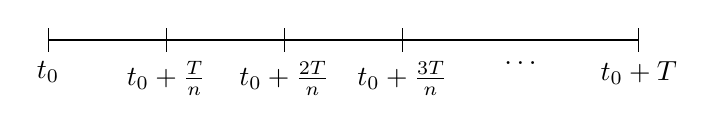
\begin{tikzpicture}[scale=1.5]
            % Intervalo [t_0, t_0 + T]
            \draw[thick] (1,0) -- (6,0);
            % Divisiones
            \foreach \x in {1, 2, 3, 4, 6} {
                \draw (\x,0.1) -- (\x,-0.1);
            }
            % Etiquetas
            \node[below] at (1,-0.1) {$t_0$};
            \node[below] at (6,-0.1) {$t_0 + T$};
            \node[below] at (2,-0.1) {$t_0 +\frac{T}{n}$};
            \node[below] at (3,-0.1) {$t_0 +\frac{2T}{n}$};
            \node[below] at (4,-0.1) {$t_0 +\frac{3T}{n}$};

            % Etiqueta de ... entre t_0 + 3T/n y t_0 + T
            \node[below] at (5,-0.1) {$\dots$};
        \end{tikzpicture}
    \]

    Ahora defino $u_n \in C (J; \, \mathbb{R}^N)$ de la siguiente manera:
    \[
        u_n(t) =
        \begin{cases}
            u_0 & t \in [t_0, t_0 + \frac{T}{n}] \\
            u_0 + \int_{t_0}^{t- \frac{T}{n}} f(s, u_n(s)) \, ds & t \in (t_0 + \frac{T}{n}, t_0 + \frac{2T}{n}] \\
            u_0 + 
            \int_{t_0}^{t_0 + \frac{T}{n}} f(s, u_n(s)) + 
            \left(
            \int_{t_0 + \frac{T}{n}}^{t - \frac{T}{n}} f(\tau, u_n(\tau)) \, d\tau 
            \right)
            \, ds & t \in (t_0 + \frac{2T}{n}, t_0 + \frac{3T}{n}] \\
            \vdots & \vdots \\
        \end{cases}
    \]
\end{proposición}